%%%%%%   TIPO DE DOCUMEN%TO: Reporte   %%%%%%
\documentclass[letterpaper,11pt]{report}
%%%%%%%%%%%%%%%%%%%%%%%%%%%%%%%%%%%%%%%%%%%%

%%%%%%%   PAQUETES   %%%%%%%
\usepackage{documento}
\usepackage{procesos}
\usepackage{requerimientos}
\usepackage[spanish]{babel}
\usepackage{graphicx}
\usepackage[utf8]{inputenc}
\usepackage{libertine}
%%%%%%%%%%%%%%%%%%%%%%%%%%%%
%%%%%%%%%%%%%%%%%%%%%%%%%%%%%%%%%%%%%%%%
%%%%%%%   INICIO DEL DOCUMENTO   %%%%%%%
%%%%%%%%%%%%%%%%%%%%%%%%%%%%%%%%%%%%%%%%
\begin{document}

    %%%%%%% Renombrar en espaNol %%%%%%
    \renewcommand{\tablename}{Tabla} %Escribe Tabla en lugar de Cuadro
    \renewcommand{\listtablename}{\'Indice de tablas} %Escribe Indeice de tablas en lugar de Indice de cuadros

    %%%%%%%   PORTADA   y RESUMEN   %%%%%%% Este es el contenido agregado de la secci\'on 2.

    %%%%%%%%%%%%%%%%%%%%%%%%%%%%%
%%%%%      PORTADA      %%%%%
%%%%%%%%%%%%%%%%%%%%%%%%%%%%%

\begin{titlepage}

    \centering %Todo centrado

    %%%%  LOGO DE LA ESCUELA   %%%%
    
\includegraphics[scale=0.17]{imagenes/escom-ipn} %Imagen para portada
    %%%%  NOMBRE DE LA ESCUELA   %%%%
    \LARGE{\\ Instituto Polit\'ecnico Nacional}
    \LARGE{\\ Escuela Superior de C\'omputo}
    
    \vspace{1cm} %Espacio vertical

    %%%%  TITULO Y NÚMERO DE TRABAJO   %%%%
    \LARGE \textbf{Sistema de Gesti\'on de Admisi\'on Escolar}
    \LARGE {\\Trabajo Terminal I No. 2019-B121}

    \vspace{1cm} %Espacio vertical

    \LARGE \textit{Que para cumplir con la opción de titulaci\'on curricular en la carrera de:}
    \LARGE \textbf{\\ Ingenier\'ia en Sistemas Computacionales}

    \vspace{1cm} %Espacio vertical

    %%%%   ALUMNOS   %%%%
   \textit{Presentan}\\
    Cervantes Moreno Christian Andr\'es \\
    Flores Altamirano Edgar \\
    L\'opez Rivera Aiko Dallane \\
    L\'opez S\'anchez Gustavo Andr\'es

    \vspace{1cm} %Espacio vertical

    %%%%   Directores   %%%%
   \textit{Directores}\\
   %%%% \bigskip%%%
    M. en C. Jos\'e Jaime L\'opez Rabad\'an \\
   %%%\bigskip  Director 2 \\%%%%
    M. en C. Verónica Agustín Dominguez
    
    

\end{titlepage} %incluye el archivo portada.tex
    %%%%%%%%%%%%%%%%%%%%%%%
%%%%    RESUMEN    %%%%
%%%%%%%%%%%%%%%%%%%%%%%

\begin{abstract}

    El Sistema de Admisión Escolar es un sistema centralizado de postulación que se realiza a través de una sistema web, en donde los aspirantes se postulan a la institución de su elección.
    En este trabajo se describen diversos procesos de admisión escolar superior, en donde las actividades que se llevan a cabo dentro de este proceso varían su orden  dependiendo las necesidades de cada institución, las cuales pueden ser: publicación de convocatoria, registro de aspirantes, aplicación de examen y publicación de resultados.  Los sistemas para la atención especializada de estos procesos son caros y no permiten variar las secuencias de actividades. 
    Por lo que se propone desarrollar un sistema que asista al proceso de admisión escolar de nivel superior, que soporte las etapas antes mencionadas pero, que permita variar el orden de éstas conforme a las necesidades de la institución, así como un módulo que permita evaluar a los aspirantes. Además se pretende cuidar aspectos de seguridad de los datos. 
    
    Palabras clave – Proceso de Admisión Escolar,  Institución de Educación Superior, Sistema Web, SCRUM.

\end{abstract}
 %Incluir resumen del documento (resumen.tex)

    %%%%%%%   INCLUIR ENCABEZADOS EN INDICES Y CAPITULOS   %%%%%%%
    \pagestyle{headings}

    %%%%%%%   NUMERACIÓN EN CONTENIDO E ÍNDICE DE TABLAS Y FIGURAS   %%%%%%%
    \pagenumbering{roman} %NUmeros romanos
    %\setcounter{page}{1} %Comienza en I por default, aquI se puedo modificar

    %%%%%%   INCLUIR CONTENIDO, INDICE DE FIGURAS E INDICE DE TABLAS   %%%%%%
    %\tableofcontents
    \tableofcontents
    \listoffigures
    \listoftables

    %%%%%%%   NUMERACION EN CAPITULOS   %%%%%%%
   % \clearpage %Para iniciar con los arAbigos
    \pagenumbering{arabic} %Numeros arabigos
    %\setcounter{page}{1} %Comienza en 1 por default, aquI se puede modificar

    %%%%%%%   INCLUYE CAPITULOS Y SECCIONES   %%%%%%%
        
        
        \chapter{Introducci\'on}
En el capítulo se presenta la explicación detallada del contenido de entrada  del Sistema de Gestión de Admisión Escolar, el cual está conformado por el contexto del trabajo, la justificación, tanto el objetivo general como el especifico, la solución propuesta y el trabajo previo.
\section{Contexto de Trabajo.}
    La era digital ha cambiado drásticamente los procesos de admisión en instituciones y universidades alrededor del mundo. La innovación, las  tecnologías en la nube, móviles y digitales están acelerando la transformación educativa, mejorando las experiencias tanto de docentes como de aspirantes [1]. Los pasos del proceso de admisión escolar usualmente son: publicación de convocatoria, registro de aspirantes, aplicación de examen y publicación de resultados, sin embargo, no todas las instituciones se apegan al mismo proceso de admisión; por lo que se propone un sistema capaz de ser configurable entre las etapas de admisión y adaptable a las instituciones.
    
    Para las instituciones de educación superior en México, el proceso de admisión consiste en elegir dentro de un conjunto de postulantes a los futuros aspirantes mejor capacitados en los programas académicos de su preferencia. Para llevar a cabo este proceso, los aspirantes a una vacante requieren de conocimientos generales relacionados al programa académico de su preferencia, además, será necesario que sigan el orden de las etapas establecidas según la institución a la que aplican.
\section{Justificación}

    De acuerdo con estadísticas de los periódicos el Universal [7] y Excélsior [8], el número de aspirantes que se postulan para ingresar al IPN y la UNAM en 2018 sumó un total de  236 mil jóvenes. Tomando como parámetro el gran número de solicitantes, resulta común que exista error en alguna de las fases del proceso de admisión, errores que, en su mayoría, fueron por actividades que son realizadas de forma manual. 
    Cuando un aspirante hace la entrega de documentos con su respectiva institución, es necesario hacer largas filas y  pasar por una cantidad definida de filtros humanos para llegar a la conclusión del proceso de recepción de documentación, pero hay un problema palpable en este hecho: los seres humanos son susceptibles a cometer errores, por tanto, existe la posibilidad de que al momento de recopilar todos los expedientes, se extravíen documentos; provocando que la institución pierda prestigio por la pérdida de información así como el tiempo perdido en las aclaraciones correspondientes. Los sistemas han sido desarrollados para evitar cometer errores, logrando resarcir esta clase de errores. Además,  sería innecesario invertir presupuesto en personal para la recepción de papeles y se evita la pérdida de tiempo para los aspirantes. En el artículo periodístico [9] se indica que los beneficios de automatizar los procesos de una empresa son: un ahorro notable al momento de utilizar recursos, una mejor inversión del tiempo, se evitan pérdidas información a causa de errores, flujo de datos mucho más eficiente y obtención de  mejores condiciones frente a la competencia.
    Pero mediante el portal de internet de INFOTECHNOLOGY [10], el costo de un software a la medida es alto ronda desde los $500,000.00 hasta $1,000,000. o más. Atendiendo estos precios la manera más viable para las instituciones es optar por algo más económico, aunque estás no se adapten totalmente a su proceso.  
    El sistema está enfocado para beneficiar a todas las instituciones automatizando este proceso de manera efectiva y segura y principalmente a aquellas en donde su proceso de admisión escolar difiere demasiado de otras, y necesitan uno económico y a la medida.
    Para hacer esto posible nos auxiliaremos de nuestros conocimientos de Base de Datos, programación en distintos lenguajes, uso de frameworks, metodologías, Ingeniería de Software, administración de tiempo y recursos, cotizar el precio un sistema, propuesta de soluciones a los problemas que se presenten, seguridad en los datos, entre otros. 

\section{Objetivo}
    Desarrollar un sistema de gestión admisión escolar que permita manejar todo un proceso de admisión a una institución, a fin de automatizar este proceso.


\subsection{Objetivos Específicos}
    
    \begin{itemize}
        \item Desarrollar una estrategia que permita configurar el orden de módulos para el sistema, para que se ajusten a la medida de cualquier institución.
        
        \item Desarrollar un módulo de registro de usuarios para facilitar su manejo en la base de datos de acuerdo a las funciones o tipo de usuario que será.
        
        \item Desarrollar el módulo de convocatorias de manera dinámica para la publicación de información que llevará a cabo cada una de las universidades.
        definir los requisitos que s ele solicitaran a un estudiante. definir y registrar 
        
        %\item Desarrollar un módulo para la gestión de plataformas de forma dinámica, para dar flexibilidad en los diversos datos a solicitar por una institución en su proceso de recepción de documentos.  
        
        \item Desarrollar un módulo de recepción de documentos para llevar a cabo la verificación y el control de cada uno de los estudiantes con base a los datos solicitados por la institución.
        
        \item Desarrollar un módulo de pagos para dar facilidad en el manejo de información referente a las condiciones de pago establecidas por cada universidad.

        \item Desarrollar un módulo de simulación de evaluación para determinar el conocimiento del estudiante con base a la evaluación propuesta por parte de la universidad.
        
        \item Desarrollar un módulo de publicación de resultados que permita conocer al aspirante el estatus de su admisión.
        
        \item Probar el funcionamiento completo y correcto del sistema para verificar que se realice todo de acuerdo a la documentación.
        
    \end{itemize}
\section{Solución propuesta}
    
    Por lo anterior se propone desarrollar un sistema en el cual se pueda configurar el orden de las etapas del proceso de admisión y se implemente un módulo de simulación de evaluación, el cual consideré únicamente preguntas de opción múltiple. Este sistema será diseñado considerando que a las instituciones educativas arrendará el servicio. 
    Además el sistema proveerá un módulo de pagos en el cual se generarán referencias para que los aspirantes la paguen en sucursal.
    Tomando en cuenta que los usuarios del sistema estarán físicamente en cualquier ubicación geográfica, el sistema deberá operar a través de la internet. En cuanto a la seguridad se pretende ofrecer al menos dos servicios de seguridad, y como mecanismos de seguridad serán la inyección de código y operación sobre el protocolo HTTPS, si bien, se pueden implementar otros mecanismos de seguridad por cuestiones de tiempo el proyecto se acotará a lo anterior.
    // ANDRÉS Y EDGAR Se propone que la arquitectura consideré la separación del código en Front-end y Back-end, y se haga uso de al menos 3 patrones de diseño.

 
\clearpage
\section{Trabajo previo}
\begin{table}[htbp!]
  \begin{center}
    \begin{figure}[H]
        \centering
        %%\caption{xxxxx}
        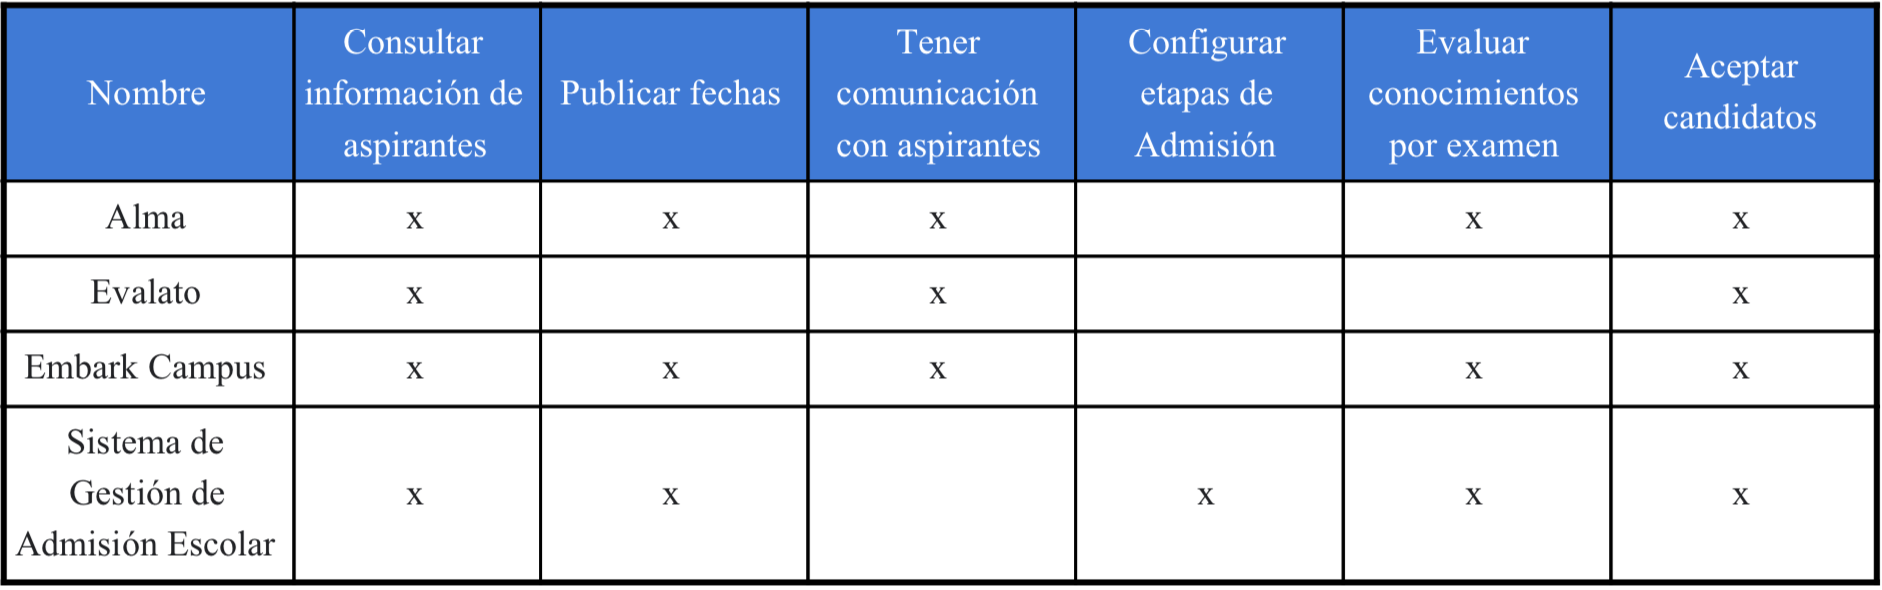
\includegraphics[width=1\textwidth]{imagenes/introduccion/tablaservicios}
    \end{figure}
    \caption{Tabla de comparación de servicios de sistemas similares disponibles en el mercado.}
    \label{tab:table1}
  \end{center}
\end{table}
\clearpage
\begin{table}[htbp!]
  \begin{center}
    \begin{figure}[H]
        \centering
        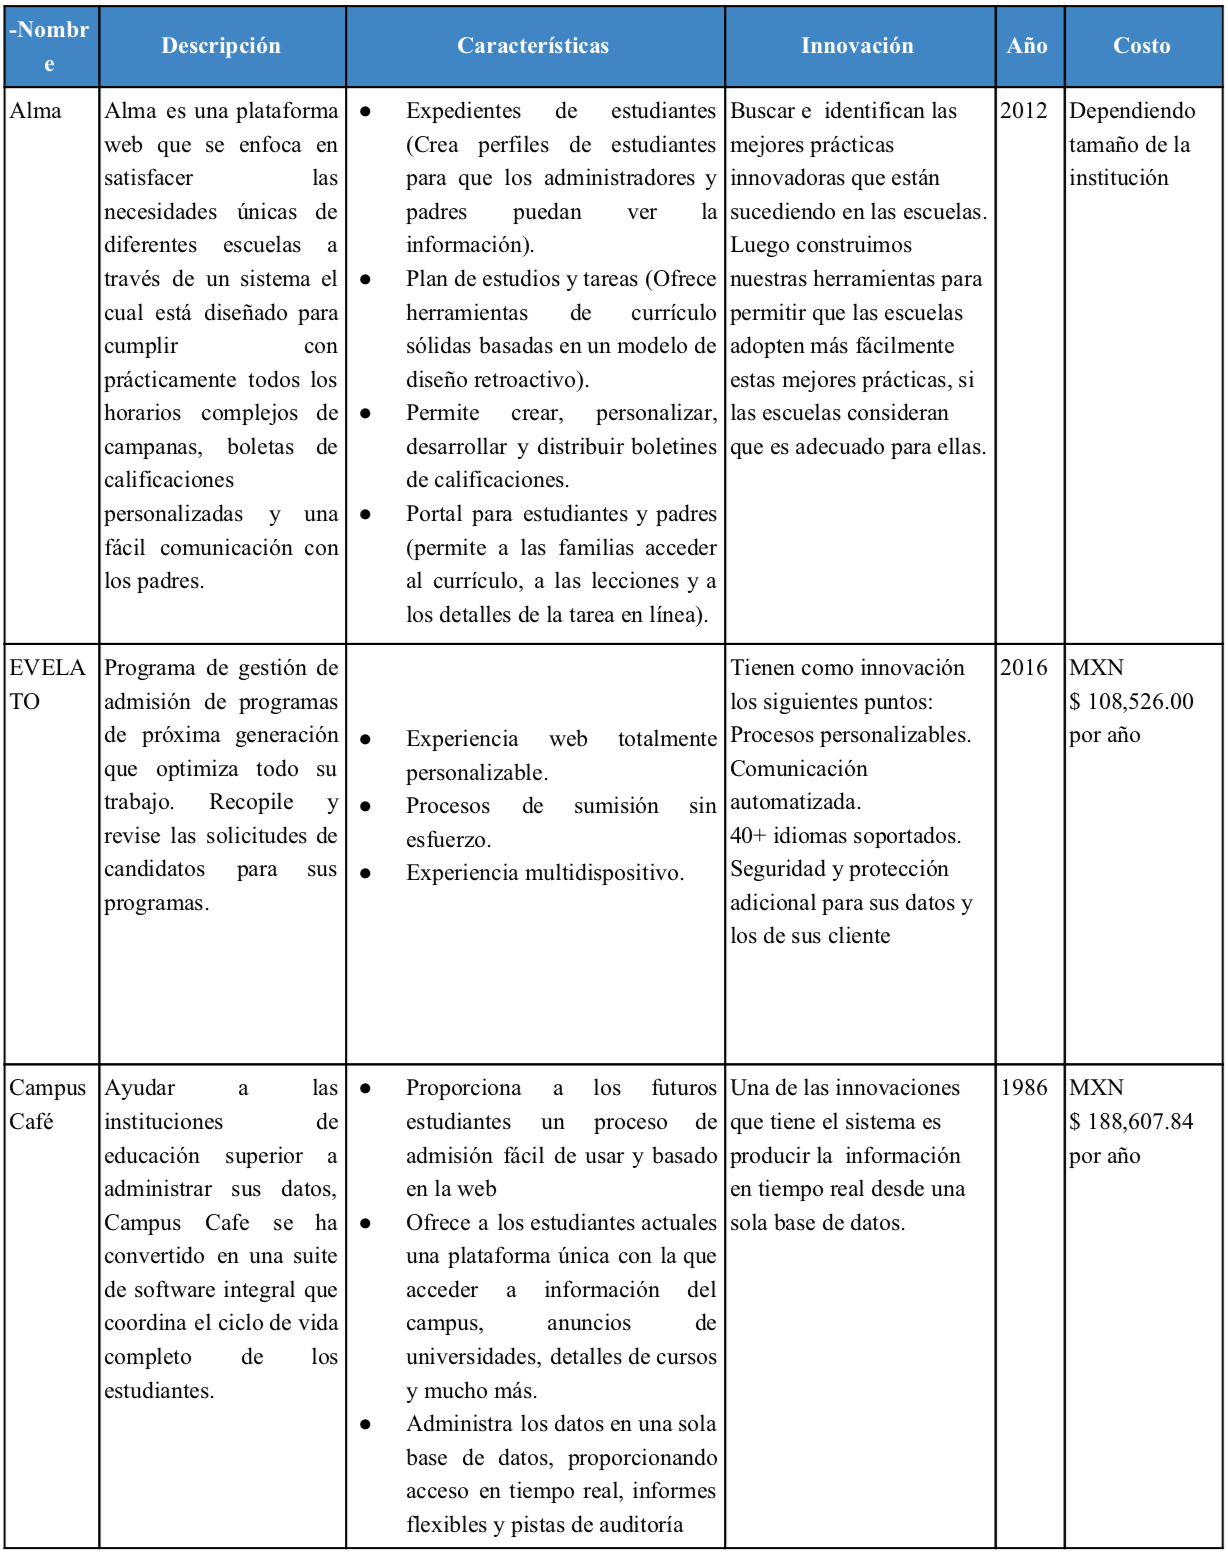
\includegraphics[width=1\textwidth]{imagenes/introduccion/tablacaracteristicas}
    \end{figure}
    \caption{Tabla de comparación de características del mercado.}
    \label{tab:table2}
  \end{center}
\end{table}


        \chapter{Marco Teórico} %CAP\'ITULO 2
    
    El marco teórico, que se desarrolla a continuación, permite conocer los conceptos básicos necesarios para el entendimiento del proyecto. 
    \section{Admisión Escolar}
    La administración escolar es un campo amplio que abarca casi cualquier tema relacionado con el funcionamiento de una institución académica, desde la gestión de un programa preescolar hasta el desarrollo de programas de doctorado.
    \section{Sistema}
    Un sistema es una disposición de partes o elementos que juntos exhiben un comportamiento o significado que los constituyentes individuales no tienen.
    Los sistemas pueden ser físicos o conceptuales, o una combinación de ambos.
    \section{Sistema Web}

    \section{Convocatoria}
    \section{Inscripción}
    \section{FireBase}
    Firebase es una tecnología que le permite crear aplicaciones web sin programación del lado del servidor, haciendo que el desarrollo sea más rápido y fácil. Es compatible con clientes web, iOS, OS X y Android. Las aplicaciones que usan Firebase pueden usar y controlar datos sin pensar en cómo se almacenan y sincronizan los datos en diferentes instancias de la aplicación en tiempo real.

    Trabajar con Firebase desde la perspectiva de un desarrollador es un beneficio maravilloso, ya que son la tecnología central del desarrollo.
    
    Ventajas:
    
    Autenticación. La autenticación de Firebase incluye un sistema de autenticación de correo electrónico / contraseña incorporado. Es compatible con OAuth2 para Facebook, Google, Twitter y GitHub. Además, el estándar Firebase se integra directamente en la base de datos Firebase para que pueda usarlo para controlar el acceso a sus datos.
    Hospedaje Firebase viene con un servicio de alojamiento fácil de usar para todos sus archivos estáticos. Funciona desde un CDN global con HTTP / 2.
    La sincronización de datos en tiempo real en todos los clientes, ya sea Android, iOS o la Web, es muy útil. Con un código mínimo, puede notificar a los usuarios de los cuadros de chat, noticias en vivo, nuevas publicaciones o solicitudes de amistad, y más.
    El código para AJS es sencillo de cualquier manera. Desde la consulta de datos hasta la integración de los inicios de sesión de Twitter, Facebook y Google+, puede implementarlos muy rápidamente con algunas características interesantes.
    Con notificaciones de actualización automática, puede sincronizar ambos sistemas sin mensajes manuales, WebSockets, etc.
    Le permite considerar flujos de datos para crear aplicaciones más escalables.
    Algunos beneficios de usar Firebase
    
    \begin{itemize}
        \item Base de datos en tiempo real de Firebase
        \item Estándar de Firebase
        \item Almacenamiento Firebase
        \item Mensaje de Firebase Cloud
        \item Notificación de Firebase
        \item Configuración remota de Firebase
        \item Informe de bloqueo de Firebase
        \item Índice de aplicaciones de Firebase
        \item Firebase Analytics
        \item Firebase Test Lab para Android
    \end{itemize}
    
    \section{Node JS}
    
    Nodo. js es una plataforma basada en el tiempo de ejecución de JavaScript de Chrome para crear fácilmente aplicaciones de red rápidas y escalables. Nodo. js utiliza un modelo de E / S sin bloqueo controlado por eventos que lo hace liviano y eficiente, perfecto para aplicaciones en tiempo real de uso intensivo de datos que se ejecutan en dispositivos distribuidos.
    \section{Angular}
    AngularJS es un marco estructural para aplicaciones web dinámicas. Le permite usar HTML como su lenguaje de plantilla y le permite extender la sintaxis de HTML para expresar los componentes de su aplicación de manera clara y sucinta. El enlace de datos de AngularJS y la inyección de dependencia eliminan gran parte del código que de lo contrario tendría que escribir. Y todo sucede dentro del navegador, lo que lo convierte en un socio ideal con cualquier tecnología de servidor.
    AngularJS es lo que habría sido HTML, si hubiera sido diseñado para aplicaciones. HTML es un gran lenguaje declarativo para documentos estáticos. No contiene mucho en cuanto a la creación de aplicaciones, y como resultado, la creación de aplicaciones web es un ejercicio de ¿qué debo hacer para engañar al navegador para que haga lo que quiero?
    %\section{Scrum}
    %\section{Evaluación}    
    %\section{Simulación}
    %\section{Arquitectura}
    %\section{Escalabilidad}
    %\section{Usalabilidad}
    %\section{Métricas}
    %\section{Mantenible}
    %\section{Metodología}    
    %\section{Regla de Negocio}
    %\section{Caso de Uso}
    %\section{Diagrama de Secuencia}
    %Andrew hace esto
    \section{Diagrama de Proceso}
    Es la representación gráfica de un conjunto de actividades, acciones o toma de decisiones interrelacionadas, caracterizadas por inputs y outputs, orientadas a obtener un resultado específico como consecuencia del valor añadido aportado por cada una de las actividades que se llevan a cabo en las diferentes etapas de dicho proceso
    \section{Interfaz de Usuario}
    Las interfaces de usuario son todo aquel espacio gráfico y físico en donde los usuarios interactúan con el software
    \section{Diagrama de componentes}
    Los diagramas de componentes son esencialmente diagramas de clase que se centran en los componentes de un sistema que a menudo se utilizan para modelar la vista de implementación estática de un sistema.
    \section{Máquina de Estados}
    Una máquina de estados es un modelo de comportamiento. Consiste en un número finito de estados, según el estado actual y una entrada dada, la máquina realiza transiciones de estado y produce salidas.
    \section{Configurable}
    Configurable es que el comportamiento de determinadas funcionalidades, la realización de determinados cálculos o la aplicación de determinadas restricciones varíe en tiempo de ejecución, también es la posibilidad de poder actualizar manualmente. 
    \section{Discente}
     Persona que recibe un aprendizaje y unos conocimientos de otra persona (generalmente de un maestro).
    \section{Pruebas de Caja Negra}
    Es una técnica de pruebas de software en la cual la funcionalidad se verifica sin tomar en cuenta la estructura interna de código, detalles de implementación o escenarios de ejecución internos en el software.
    \section{Gestión}
    Hace la referencia a la administración de recursos, sea dentro de una institución estatal o privada, para alcanzar los objetivos propuestos por la misma.
    \section{Inyección de Código}
     Es el proceso de introducir a un programa ó sistema software una serie de instrucciones que no formaban parte de la composición original del  programa/sistema, provocando modificaciones en el funcionamiento original del programa/sistema, y en su rendimiento .
    \section{Integridad}%Seguridad
     Es la cualidad que posee un documento que no ha sido alterado y que además permite comprobar que no sea manipulado el documento original.
    \section{Autenticación}%S
    Es la comprobación de la identidad de una persona o de un objeto
    \section{Confidencialidad}%S
    Se conoce en derecho como una comunicación privilegiada, la cual se define como un intercambio de información entre dos personas en una relación entre el profesional y su cliente, en la cual la relación confidencial es expresamente reconocida por ley. 
    \section{Patrones de diseño}
    \section{MVVM}
    MVVM es una arquitectura desarrollada por Microsoft alrededor de 2004, cuando también se creó Windows Presentation Foundation.
    \section{Protocolo HTTPS}
    El Protocolo seguro de transferencia de hipertexto es un protocolo de aplicación basado en el protocolo HTTP, destinado a la transferencia segura de datos de hipertexto, es decir, es la versión segura de HTTP.
    
    
        \chapter{Análisis}
En este capitulo se presenta todo el análisis que conlleva este sistema, en el cual se incluye la metodología, diagramas de procesos, diagramas de procesos, reglas de negocio, mensajes, tanto requerimientos funcionales como no funcionales y finalmente los casos de uso. 
    \section{Metodología}
\pagebreak
    \section{Diagramas de Procesos}

\begin{BPMN}{MCD}{Creación de Requisitos para Documentación}{}
    \PCitem{Participantes}{\begin{itemize}
    		\item Docentes de la Academias	
    		\item Comité de Evaluación Curricular
    		\item Colegio de Profesores
    		\item Dirección General 
    \end{itemize}}
    \PCitem{Objetivo}{La elaboración o rediseño  de las Unidades de Aprendizaje, ya sea de forma individual o en paquetes, que pertenecen a un Plan de Estudios en un Programa Académico del IPN.}
    \PCitem{Interrelación con otros procesos}{
    \begin{itemize}
    	\item Entrada: Requisito de rediseñar o diseñar una nueva Unidad de Aprendizaje en un Plan de Estudios.
    	\item Salida: Tiras de Unidades de Aprendizaje en un Plan de Estudios.
	\end{itemize}
    }
    \PCitem{Entradas}{Plantillas de creación de Unidades de Aprendizaje}
    \PCitem{Consumidores}{Unidad Académica}
    \PCitem{Salidas}{Tiras de unidades de aprendizaje}
    \PCitem{Precondiciones}{Carga de resumen del Plan de Estudios}
    \PCitem{Postcondiciones}{Finalización del diseño o rediseño de un Programa Académico}
    \PCitem{Tipo}{Operativo}
\end{BPMN}
En la figura \hyperref[fig:MCD]{BPMN-02 Proceso para la creación de una Unidad de Aprendizaje}

\begin{figure}[H]
        \centering
        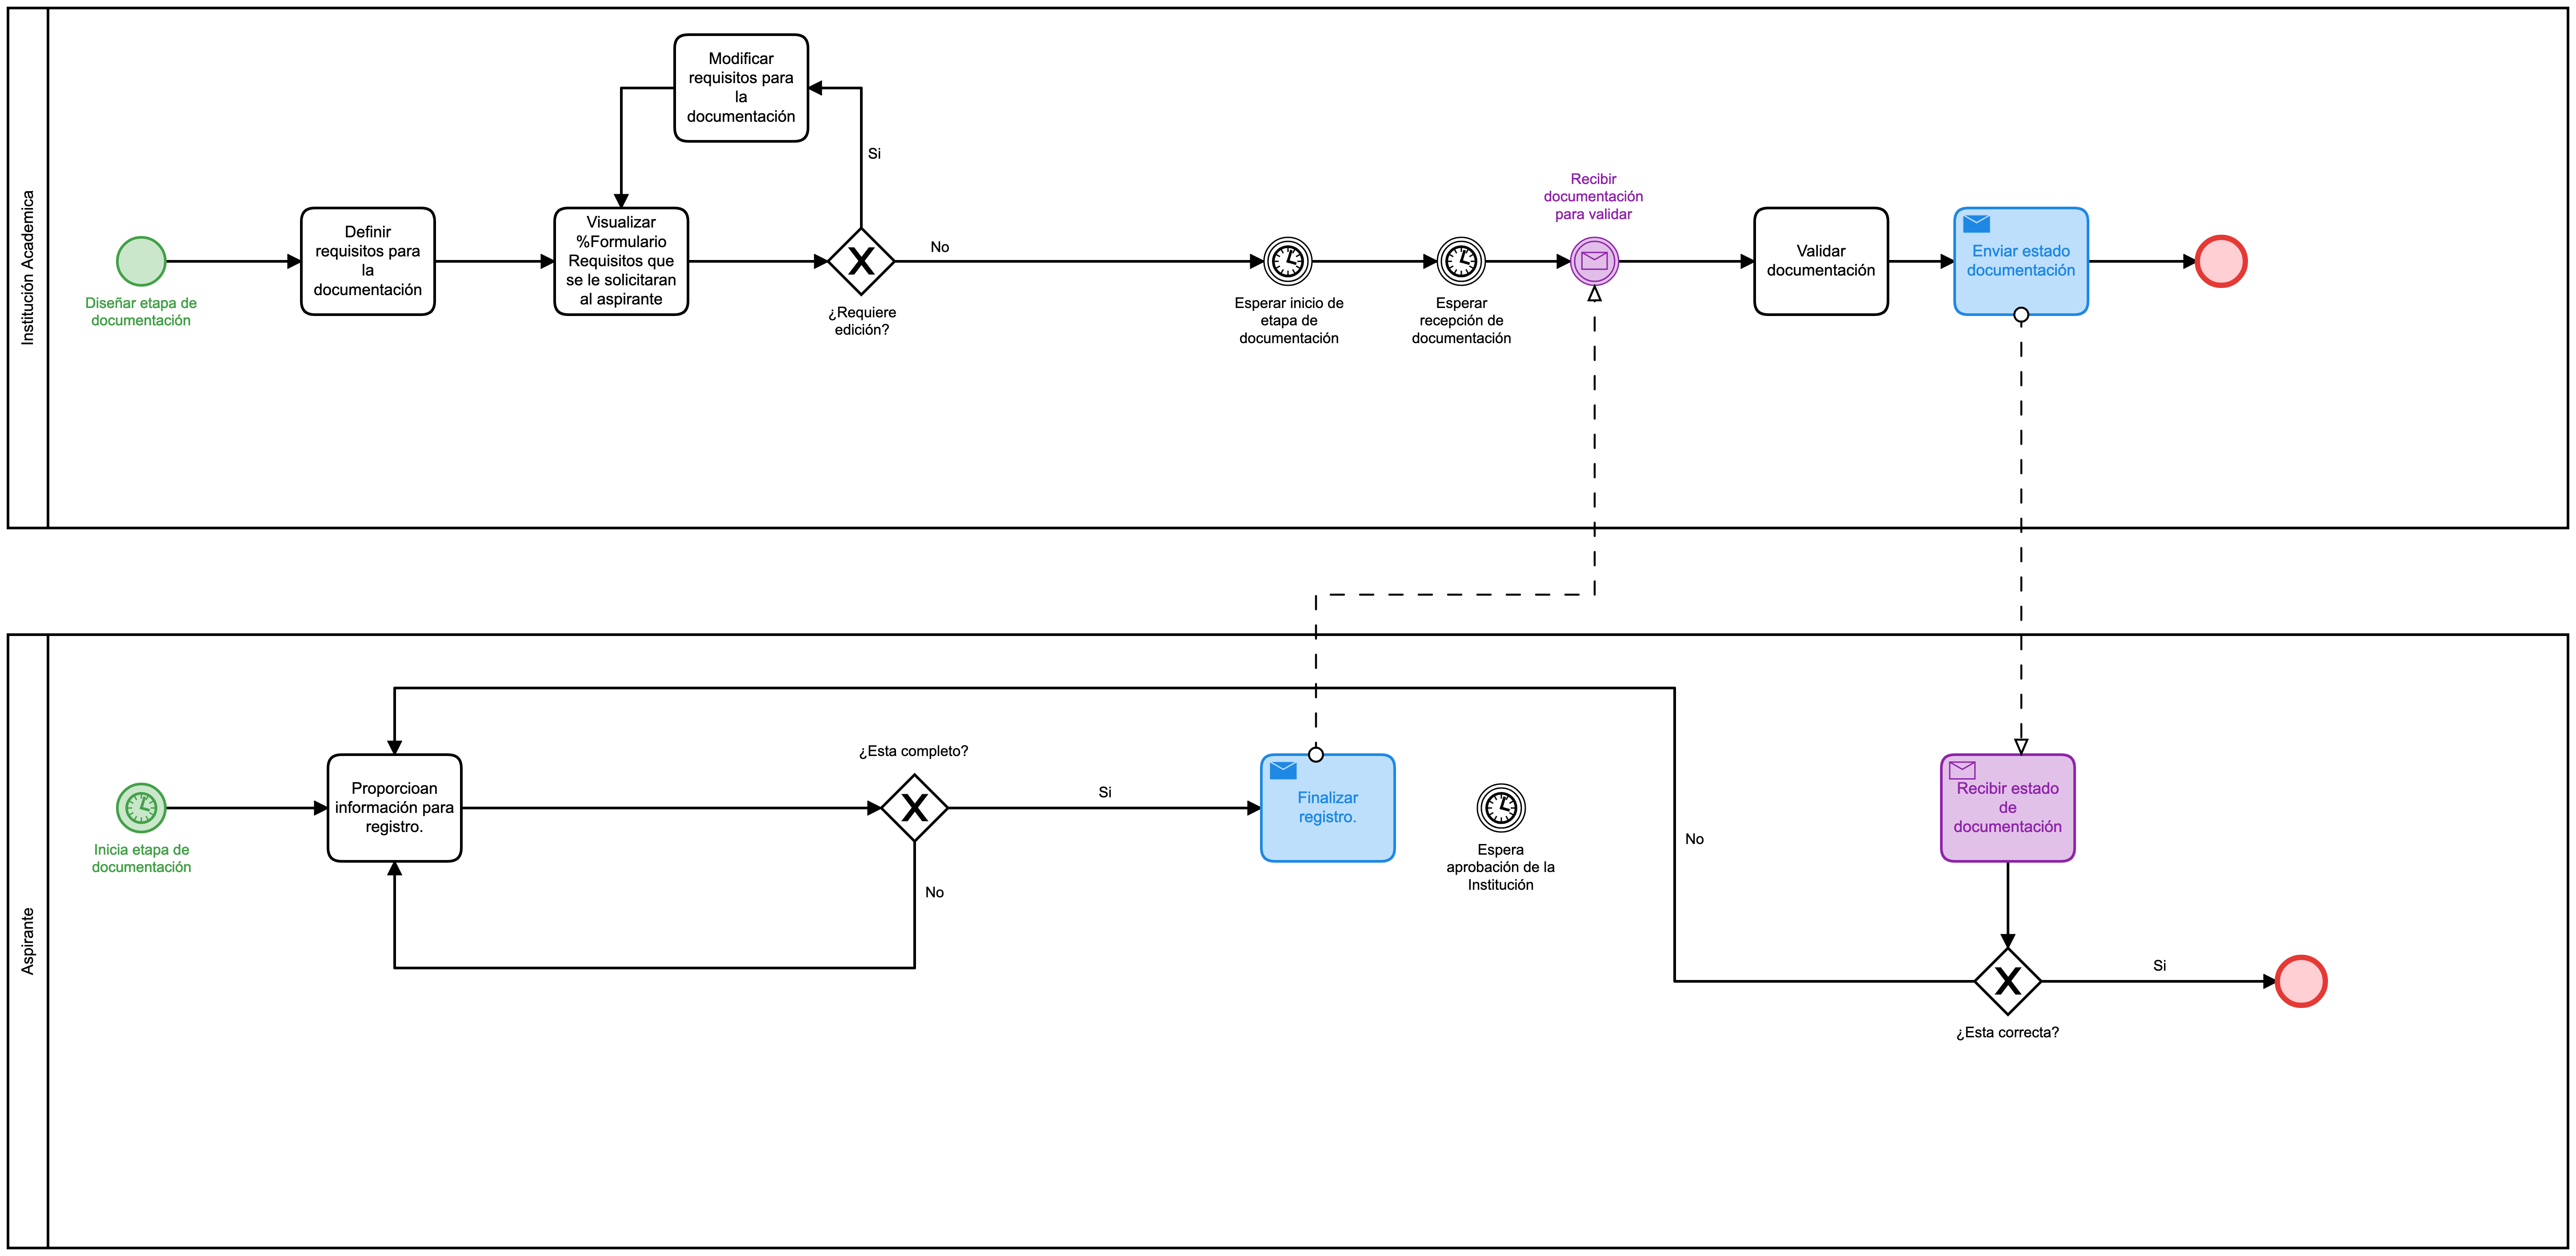
\includegraphics[width=1\textwidth]{TTI_2019-A055/imagenes/procesos/procesoDocumentacion.png}
        \caption{Proceso de Requisitos para Documentación.}
        \label{fig:MCD}
    \end{figure}
\newpage
\begin{itemize}
	\item \textbf{Elaborar instrumento para conocer el estado actual de la unidad de aprendizaje:} Se realiza la evaluación curricular dentro de la Unidad Académica para determinar la viabilidad de actualizar la Unidad de Aprendizaje.
	\item \textbf{Evaluación cuantitativa:}
	\item \textbf{Proporcionar instrumentos a los docentes:} Enviar los instrumentos y resultados de la evaluación curricular a los docentes encargados de la realización de la Unidad de Aprendizaje.
	\item \textbf{Elaborar informe:} Los docentes encargados, con base a los resultados obtenidos en la evaluación, realizan el informe del estado actual de la Unidad de Aprendizaje.
	\item \textbf{Elaborar diagnóstico:} Se determina si se aprueba o se rechazan los procesos de diseño o rediseño de la Unidad de Aprendizaje, según el informe del estado actual y la evaluación realizada.
	\item \textbf{Elaborar la "Descripción general de la Unidad de Aprendizaje":} Iniciar los procesos de rediseño o diseño de la Unidad de Aprendizaje. Se describe la asignatura.
	
	\item \textbf{Diseñar el programa de la asignatura:} Se inician los procesos de llenado de los programas sintéticos y en extenso de la Unidad de Aprendizaje.
	\item \textbf{Enviar a revisión:}  Los docentes envían los programas de la asignatura al Colegio de Profesores para su revisión.
	\item \textbf{Analizar el programa de la asignatura:} Se inician los trabajos de revisión de los programas sintéticos y en extenso de la Unidad de Aprendizaje por parte del Colegio de Profesores.
	
	\item \textbf{Enviar Unidad de Aprendizaje:}  Una vez aprobados los programas de la Unidad de Aprendizaje, se envían al Comité de Evaluación Curricular. Culmina el proceso.
	\item \textbf{Enviar ajustes:} Si existen correcciones o notas respecto a los programas de la Unidad de Aprendizaje, éstos se envían junto a ésta de vuelta a los docentes para ser atendidos.    
\end{itemize}

\pagebreak

% Procesos que yo debo de hacer
\begin{BPMN}{MGE}{Proceso del Modulo de Gestión de Etapas}{El proceso consiste en gestionar o bien configurar el orden de las etapas del proceso de admisión escolar las cuales son: convocatoria, recepción de documentos, pagos, evaluación y publicación de resultados, el único actor que interactúa en este proceso es el administrador root el cual tiene como tareas seleccionar las etapas que desee, ordenarlas, definir el periodo de cada una de las etapas y visualizarlas.}
    \PCitem{Participantes}{\begin{itemize}
    		\item Administrador Root.
    \end{itemize}}
    \PCitem{Objetivo}{Desarrollar una estrategia que permita configurar el orden de módulos para el sistema, para que se ajusten a la medida de cualquier institución.}
    \PCitem{Interrelación con otros procesos}{
    \begin{itemize}
    	\item Entrada: Iniciar Sesión.
    	\item Salida: El primer modulo de la etapa de proceso de admisión escolar que el administrador haya asignado..
	\end{itemize}
	}
    \PCitem{Entradas}{}
    \PCitem{Consumidores}{}
    \PCitem{Salidas}{Etapas configuradas.}
    \PCitem{Precondiciones}{El administrador root debe de iniciar sesión.}
    \PCitem{Postcondiciones}{Finalización de la seleción y orden de las etapas de proceso de admisión escolar.}
    \PCitem{Tipo}{Operativo}
\end{BPMN}
En la figura \hyperref[fig:MGE]{BPMN-02 Proceso para la creación de una Unidad de Aprendizaje}

\begin{figure}[H]
        \centering
        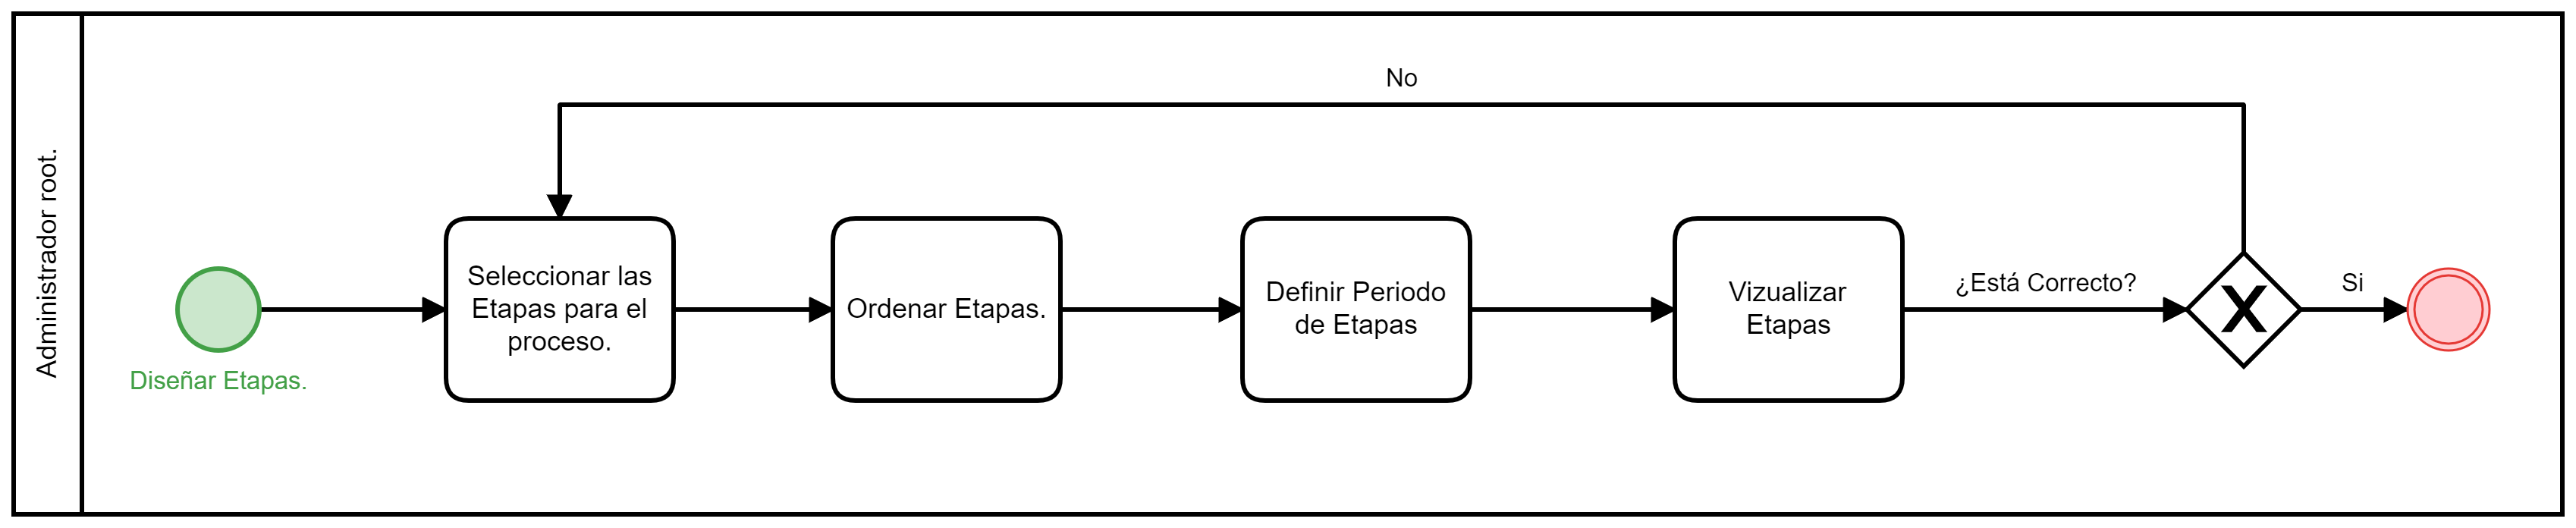
\includegraphics[width=1\textwidth]{TTI_2019-A055/imagenes/procesos/procesoGestionDeEtapas.png}
        \caption{Proceso de Gestión de Etapas.}
        \label{fig:MGE}
    \end{figure}

\begin{itemize}
	\item \textbf{Elaborar instrumento para conocer el estado actual de la unidad de aprendizaje:} Se realiza la evaluación curricular dentro de la Unidad Académica para determinar la viabilidad de actualizar la Unidad de Aprendizaje.
	\item \textbf{Evaluación cuantitativa:}
	\item \textbf{Proporcionar instrumentos a los docentes:} Enviar los instrumentos y resultados de la evaluación curricular a los docentes encargados de la realización de la Unidad de Aprendizaje.
	\item \textbf{Elaborar informe:} Los docentes encargados, con base a los resultados obtenidos en la evaluación, realizan el informe del estado actual de la Unidad de Aprendizaje.
	\item \textbf{Elaborar diagnóstico:} Se determina si se aprueba o se rechazan los procesos de diseño o rediseño de la Unidad de Aprendizaje, según el informe del estado actual y la evaluación realizada.
	\item \textbf{Elaborar la "Descripción general de la Unidad de Aprendizaje":} Iniciar los procesos de rediseño o diseño de la Unidad de Aprendizaje. Se describe la asignatura.
	
	\item \textbf{Diseñar el programa de la asignatura:} Se inician los procesos de llenado de los programas sintéticos y en extenso de la Unidad de Aprendizaje.
	\item \textbf{Enviar a revisión:}  Los docentes envían los programas de la asignatura al Colegio de Profesores para su revisión.
	\item \textbf{Analizar el programa de la asignatura:} Se inician los trabajos de revisión de los programas sintéticos y en extenso de la Unidad de Aprendizaje por parte del Colegio de Profesores.
	
	\item \textbf{Enviar Unidad de Aprendizaje:}  Una vez aprobados los programas de la Unidad de Aprendizaje, se envían al Comité de Evaluación Curricular. Culmina el proceso.
	\item \textbf{Enviar ajustes:} Si existen correcciones o notas respecto a los programas de la Unidad de Aprendizaje, éstos se envían junto a ésta de vuelta a los docentes para ser atendidos.    
\end{itemize}


    \begin{figure}[H]
        \centering
        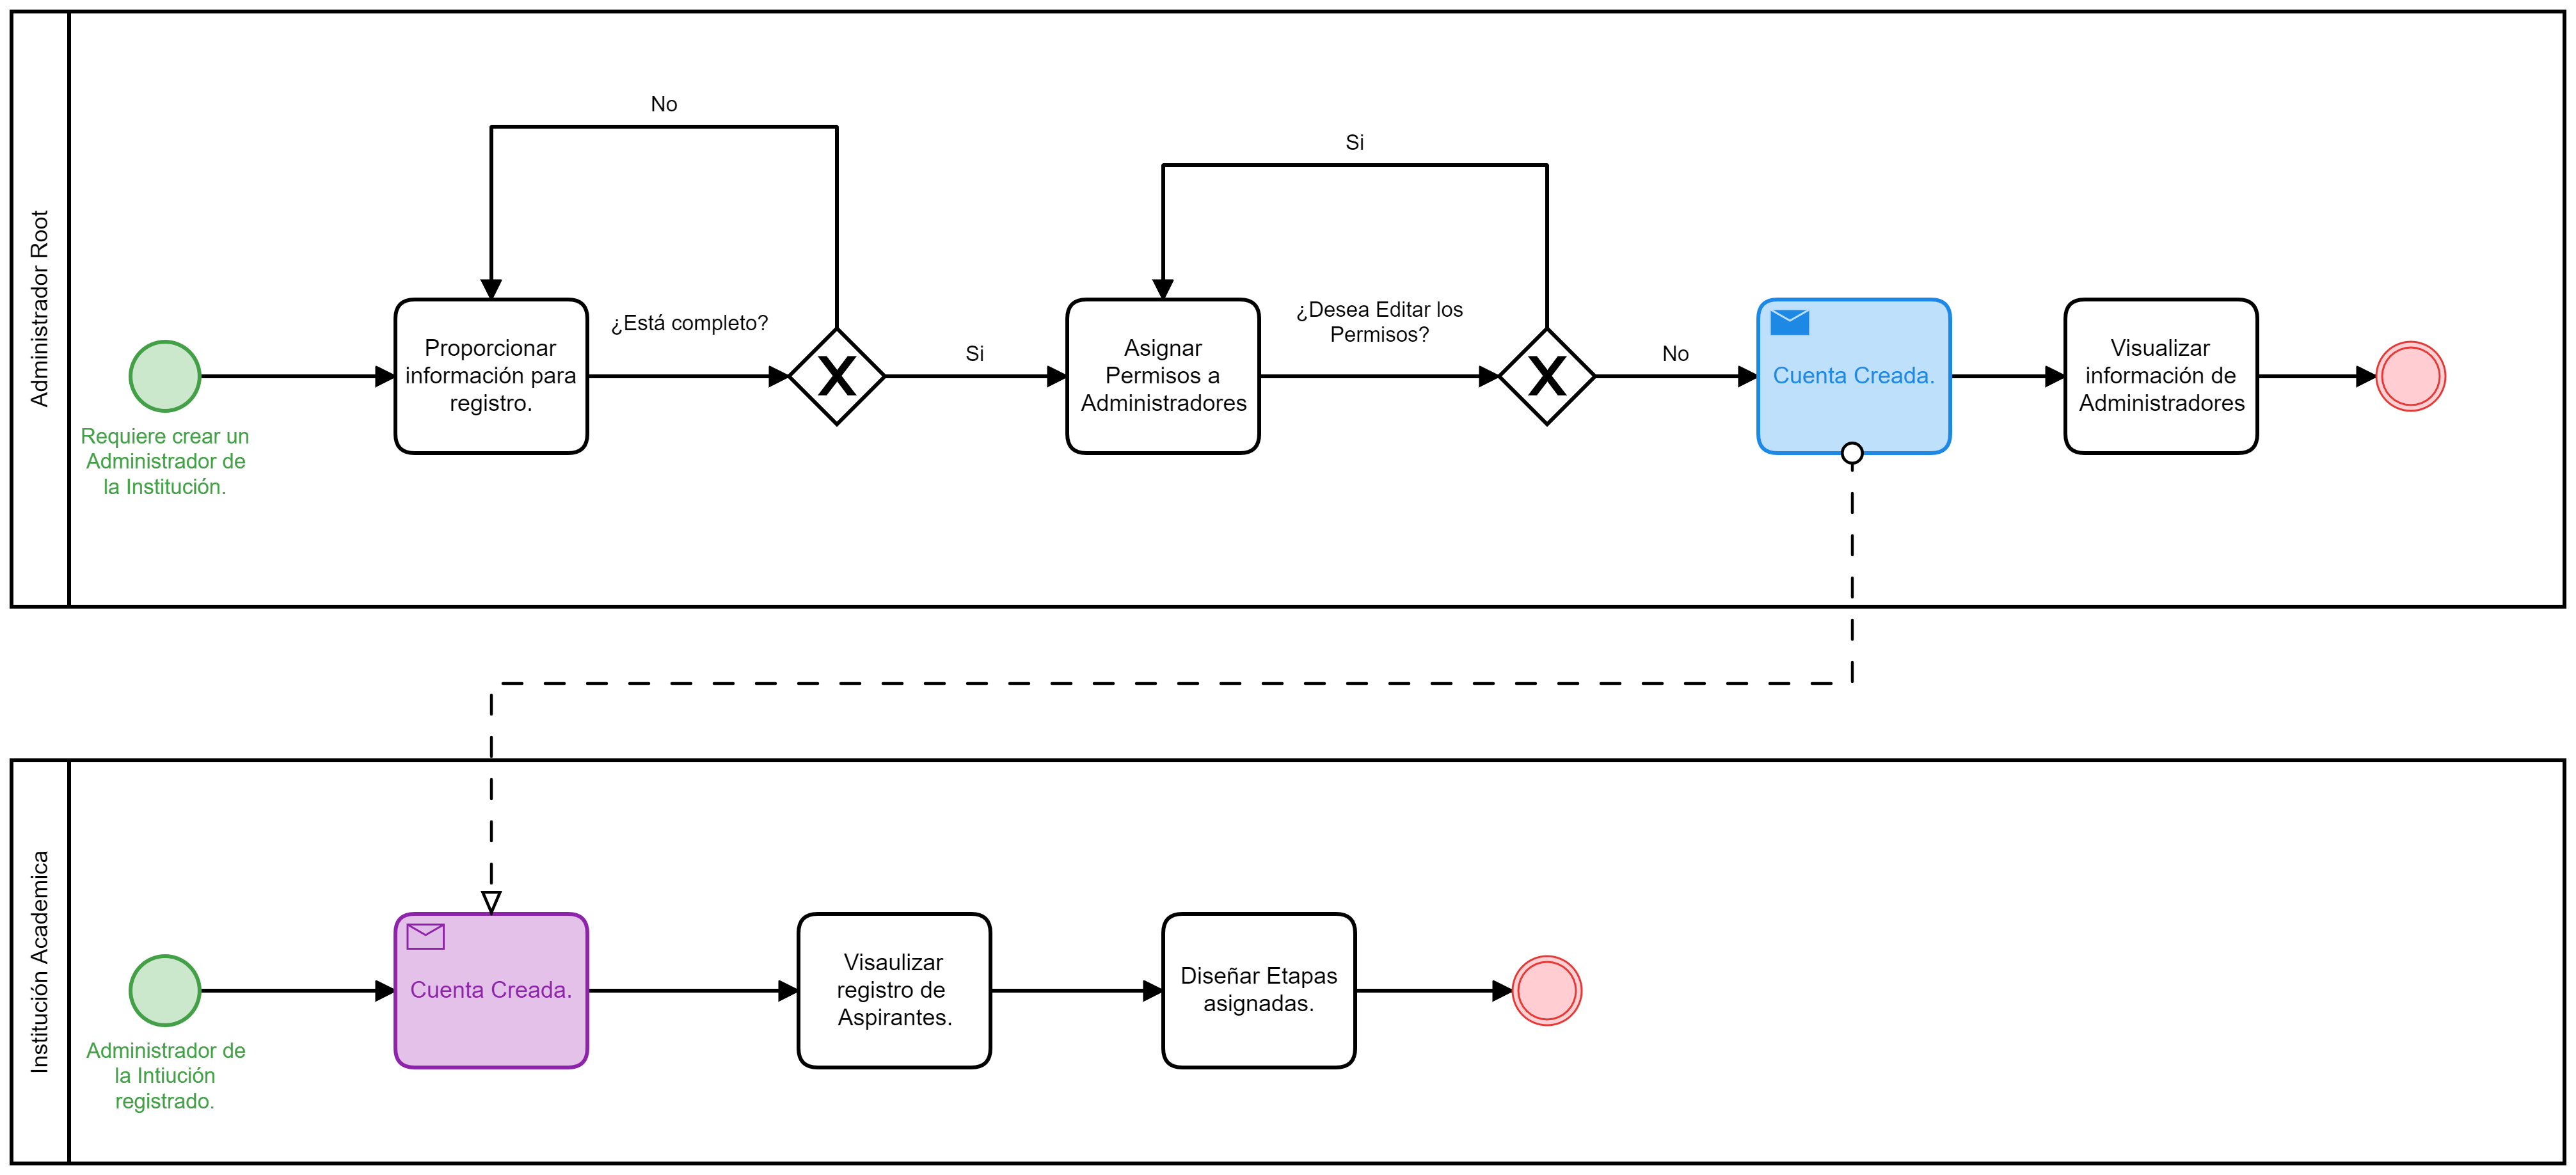
\includegraphics[width=1\textwidth]{TTI_2019-A055/imagenes/procesos/procesoGestionDeUsuarios.png}
        \caption{Proceso de Gestión de Usuarios.}
    \end{figure}

    \section{Reglas de Negocio}
\begin{BussinesRule}{BR1}{}
    \BRitem[Tipo:]
    \BRitem[Clase:]
    \BRitem[Nivel:]
    \BRitem[Descripción:]Para la creación del formulario  al menos debe existir un requisito.
    
\end{BussinesRule}
%----------------------------------BR --------------------------------------%
\begin{BussinesRule}{BR2}{}
    \BRitem[Tipo:]
    \BRitem[Clase:]
    \BRitem[Nivel:]
    \BRitem[Descripción:]Un requisito deberá conformarse de nombre y tipo de dato.
    
\end{BussinesRule}
%----------------------------------BR --------------------------------------%
\begin{BussinesRule}{BR3}{}
    \BRitem[Tipo:]
    \BRitem[Clase:]
    \BRitem[Nivel:]
    \BRitem[Descripción:]El nombre del tipo de dato es alfanumérico.
    
\end{BussinesRule}
%----------------------------------BR --------------------------------------%
\begin{BussinesRule}{BR4}{}
    \BRitem[Tipo:]
    \BRitem[Clase:]
    \BRitem[Nivel:]
    \BRitem[Descripción:]Los tipos de datos que se podrán introducir serán campo, archivo, de selección y fecha. 
    
\end{BussinesRule}
%----------------------------------BR --------------------------------------%
\begin{BussinesRule}{BR5}{}
    \BRitem[Tipo:]
    \BRitem[Clase:]
    \BRitem[Nivel:]
    \BRitem[Descripción:]El tipo de dato campo solo podrá ser de texto y número
    
\end{BussinesRule}
%----------------------------------BR --------------------------------------%
\begin{BussinesRule}{BR6}{}
    \BRitem[Tipo:]
    \BRitem[Clase:]
    \BRitem[Nivel:]
    \BRitem[Descripción:]El tipo de dato archivo solo podrá ser una imagen con extensión png y jpg, o  pdf.
    
\end{BussinesRule}
%----------------------------------BR --------------------------------------%
\begin{BussinesRule}{BR7}{}
    \BRitem[Tipo:]
    \BRitem[Clase:]
    \BRitem[Nivel:]
    \BRitem[Descripción:]El tipo de dato de selección podrá ser con opción única o múltiple.
    
\end{BussinesRule}
%----------------------------------BR --------------------------------------%
\begin{BussinesRule}{BR8}{}
    \BRitem[Tipo:]
    \BRitem[Clase:]
    \BRitem[Nivel:]
    \BRitem[Descripción:]En el tipo de dato de fecha se deberá seleccionar el rango de tiempo.
    
\end{BussinesRule}
%----------------------------------BR --------------------------------------%
\begin{BussinesRule}{BR9}{}
    \BRitem[Tipo:]
    \BRitem[Clase:]
    \BRitem[Nivel:]
    \BRitem[Descripción:]Creado el requisito, toda las caracteristicas  se podrán editar a excepción del tipo de dato.
    
\end{BussinesRule}
%----------------------------------BR --------------------------------------%
\begin{BussinesRule}{BR10}{}
    \BRitem[Tipo:]
    \BRitem[Clase:]
    \BRitem[Nivel:]
    \BRitem[Descripción:]Un requisito tendrá la opción de ser obligatorio o no.
    
\end{BussinesRule}
%----------------------------------BR --------------------------------------%
\begin{BussinesRule}{BR11}{}
    \BRitem[Tipo:]
    \BRitem[Clase:]
    \BRitem[Nivel:]
    \BRitem[Descripción:]En la vista previa del formulario,  se podrá verificar mediante el botón finalizar. ????
    
\end{BussinesRule}
%----------------------------------BR --------------------------------------%
\begin{BussinesRule}{BR12}{}
    \BRitem[Tipo:]
    \BRitem[Clase:]
    \BRitem[Nivel:]
    \BRitem[Descripción:]En caso de recibir una validación aprobatoria, se deberá esperar a la siguiente etapa del proceso.
    
\end{BussinesRule}
%----------------------------------BR --------------------------------------%
\begin{BussinesRule}{BR13}{}
    \BRitem[Tipo:]
    \BRitem[Clase:]
    \BRitem[Nivel:]
    \BRitem[Descripción:]En caso de recibir una validación desaprobada, solo se habilitara el requisito a modificar y la opción de volver a enviar formulario.
    
\end{BussinesRule}
%----------------------------------BR --------------------------------------%
\begin{BussinesRule}{BR14}{}
    \BRitem[Tipo:]
    \BRitem[Clase:]
    \BRitem[Nivel:]
    \BRitem[Descripción:]La revisión para validación de un alumno solo se hará por un adminitsrador  de la institución a la vez.
    
\end{BussinesRule}
%----------------------------------BR --------------------------------------%
\begin{BussinesRule}{BR15}{}
    \BRitem[Tipo:]
    \BRitem[Clase:]
    \BRitem[Nivel:]
    \BRitem[Descripción:]La pantalla de visualizar alumnos contendrá una tabla con nombre(s) del alumno, status de validación y acciones.
    
\end{BussinesRule}
%----------------------------------BR --------------------------------------%
\begin{BussinesRule}{BR16}{}
    \BRitem[Tipo:]
    \BRitem[Clase:]
    \BRitem[Nivel:]
    \BRitem[Descripción:]En caso de que todos los requisitos estén completos y validados, se enviara la notificación a alumno de esto, al igual que si no están validados, se mandara la notificación de que requisito(s) corregir, anexando el comentario del error. 
    
\end{BussinesRule}
%----------------------------------BR --------------------------------------%
\begin{BussinesRule}{BR17}{}
    \BRitem[Tipo:]
    \BRitem[Clase:]
    \BRitem[Nivel:]
    \BRitem[Descripción:]
    
\end{BussinesRule}
%----------------------------------BR --------------------------------------%
\begin{BussinesRule}{BR18}{}
    \BRitem[Tipo:]
    \BRitem[Clase:]
    \BRitem[Nivel:]
    \BRitem[Descripción:]
    
\end{BussinesRule}
%----------------------------------BR --------------------------------------%
\begin{BussinesRule}{BR19}{Máquina de Estados de una Tarea.}
    \BRitem[Tipo:] Flujo.
    \BRitem[Clase:] Habilitadora.
    \BRitem[Nivel:] Control.
    \BRitem[Descripción:] Según el estado de la Tarea son los permisos de quien puede modificar la información relacionada con esta.
     Tener un mayor control sobre la información.
    \BRitem[Ejemplo Positivo:] La Tarea de registrar Mapa Curricular se aprobó después de que el analista y el jefe la revisaran.
    \BRitem[Ejemplo Negativo:] La Tarea de registrar Unidad de Aprendizaje se empezó a revisar antes de que terminara su registro.
\end{BussinesRule}
%----------------------------------BR --------------------------------------%
\begin{BussinesRule}{BR20}{Aprobación de Tareas.}
    \BRitem[Tipo:] Flujo.
    \BRitem[Clase:] Habilitadora.
    \BRitem[Nivel:] Control.
    \BRitem[Descripción:] Una Tarea es aprobada si al terminar de revisar no contiene comentarios.
     Poder saber cuando una tarea a finalizado.
    \BRitem[Ejemplo Positivo:] El Jefe de Innovación Educativa no agrego comentarios por lo que se aprueba.
    \BRitem[Ejemplo Negativo:] El Jefe de Innovación Educativa agrega comentario y aun así se aprueba el documento.
\end{BussinesRule}
%----------------------------------BR --------------------------------------%
\begin{BussinesRule}{BR21}{Aprobación de Tareas Seccionada.}
    \BRitem[Tipo:] Condición.
    \BRitem[Clase:] Habilitadora.
    \BRitem[Nivel:] Control.
    \BRitem[Descripción:]
    \BRitem[Sentencia:] Una tarea puede ser aprobada parcialmente y las secciones aprobadas no pueden ser modificadas.
     Evitar modificaciones en una sección ya aprobada.
    \BRitem[Ejemplo Positivo:] Una sección ya ha sido aprobada y no se hacen modificaciones.
    \BRitem[Ejemplo Negativo:] Una sección es aprobada y fue modificada.
\end{BussinesRule}
%----------------------------------BR --------------------------------------%
\begin{BussinesRule}{BR22}{Rechazo de Tareas.}
    \BRitem[Tipo:] Flujo.
    \BRitem[Clase:] Habilitadora.
    \BRitem[Nivel:] Control.
    \BRitem[Descripción:] Una Tarea es rechazada si al terminar de revisar contiene comentarios.
     Poder saber cuando una tarea debe volver al estado de Registro.
    \BRitem[Ejemplo Positivo:] El Jefe de Innovación Educativa agrego comentarios por lo que se rechaza.
    \BRitem[Ejemplo Negativo:] Ni el Jefe de Innovación Educativa ni el Analista agregaron comentarios y aun así se aprobó.
\end{BussinesRule}
%----------------------------------BR --------------------------------------%
\begin{BussinesRule}{BR23}{Tiempos de entregas.}
    \BRitem[Tipo:] Integridad.
    \BRitem[Clase:] Cronometrado.
    \BRitem[Nivel:] Control.
    \BRitem[Descripción:] Una tarea debe entregarse en la fecha indicada por el jefe de desarrollo e innovación curricular.
     Se tiene un control en las entregas de tareas.
    \BRitem[Ejemplo Positivo:] Una propuesta de unidad de aprendizaje puede ser revisada por un analista solo en el tiempo establecido.
    \BRitem[Ejemplo Negativo:] Una propuesta de unidad de aprendizaje puede ser revisada por un analista en cualquier momento.
\end{BussinesRule}
%----------------------------------BR --------------------------------------%
\begin{BussinesRule}{BR24}{Todos los datos solicitados son obligatorios.}
    \BRitem[Tipo:] Regla de Operación.
    \BRitem[Clase:] Habilitadora.
    \BRitem[Nivel:] Control.
    \BRitem[Descripción:] Los campos solicitados, no se pueden ser dejados en blanco.
    \BRitem[Sentencia:]
    \BRitem[Motivación: ]Que la base de datos esté siempre en un estado consistente.
    \BRitem[Ejemplo Positivo:] El usuario ingresa todos los datos solicitados y prosigue con su operación.
    \BRitem[Ejemplo Negativo: ]El usuario deja campos vacios y el sistema le permite continuar.
\end{BussinesRule}
%----------------------------------BR --------------------------------------%
\begin{BussinesRule}{BR25}{El correo electrónico del empleado es único.}
    \BRitem[Tipo: ]Relación.
    \BRitem[Clase: ]Habilitadora.
    \BRitem[Nivel: ]Control.
    \BRitem[Descripción:] Cada una de las cuentas de los empleados registrados en el sistema cuentan con un correo electrónico único.
    \BRitem[Motivación: ]Poder identificar a los usuarios.
    \BRitem[Ejemplo Positivo:] El Empleado Juan Perez tiene una correo electrónico juanp@ipn.mx  y el empleado Armando López Doriga tiene un correo electrónico armlop@ipn.mx.
    \BRitem[Ejemplo Negativo:] El Empleado Juan Perez tiene una correo electrónico juanp@ipn.mx  y el empleado Armando López Doriga tiene un correo electrónico juanp@ipn.mx.
\end{BussinesRule}
%----------------------------------BR --------------------------------------%

\begin{BussinesRule}{BR26}{Debe existir al menos un criterio de evaluación para una Unidad de Aprendizaje.}
    \BRitem[Tipo:] Regla de integridad estructural.
    \BRitem[Clase:] Habilitadora.
    \BRitem[Nivel:] Control.
    \BRitem[Descripción:] Para cada Unidad de Aprendizaje debe existir al menos un criterio de evaluación cuyo porcentaje asociado sería de 100\%, sin embargo, puede tener tantos criterios como el docente decida.
     Que el docente que imparta dicha Unidad de Aprendizaje tenga al menos un referente para evaluar a sus alumnos.
    \BRitem[Ejemplo positivo:] La Unidad de Aprendizaje ``Ingeniería de Sofware'' tiene como único criterio de evaluación el desarrollo de un proyecto cuyo porcentaje equivale al 100\% de la calificación del alumno.
\end{BussinesRule}
%----------------------------------BR --------------------------------------%
\begin{BussinesRule}{BR27}{La suma de los porcentajes de cada evaluación debe ser igual a 100\%.}
    \BRitem[Tipo:] Regla de operación.
    \BRitem[Clase:] Habilitadora.
    \BRitem[Nivel:] Control.
    \BRitem[Descripción:] La suma total de los porcentajes de cada evaluación registrada por el docente, debe ser exactamente igual al 100\%.
     Que exista coherencia al momento de evaluar y que el alumno pueda identificar de dónde proviene su calificación.
    \BRitem[Ejemplo positivo:] Las evaluaciones registradas para la Unidad de Aprendizaje ``Ingeniería de Software'' son:
        \begin{itemize}
            \item 20\% Examen oral.
            \item 20\% Tareas.
            \item 60\% Proyecto final.
        \end{itemize}
        En total, los porcentajes suman el 100\% de la calificación del alumno.
\end{BussinesRule}
%----------------------------------BR --------------------------------------%
   \begin{BussinesRule}{BR28}{Dirección web del sistema.}
     \BRitem[Tipo:] Flujo.
     \BRitem[Clase:] Habilitadora.
     \BRitem[Nivel:] Control.
     \BRitem[Descripción:] La dirección web a la cual tendrán que ingresar los usuarios en su navegador para acceder al sistema es la siguiente: \url{https://sgae-escom.firebaseapp.com/#/}
      Informar a los usuarios cómo acceder al sistema una vez puesto en línea.
  \end{BussinesRule}
 %----------------------------------BR --------------------------------------%
   \begin{BussinesRule}{BR29}{Verificación de formularios al momento.}
     \BRitem[Tipo:]  Estímulo y respuesta.
     \BRitem[Clase:] Habilitadora.
     \BRitem[Nivel:] Control.
     \BRitem[Descripción:] El sistema realiza las verificaciones conforme al Modelo de Datos mientras el Usuario ingresa los datos.
      Evitar inconsistencias en los datos.
  \end{BussinesRule}
  %----------------------------------BR --------------------------------------%
\begin{BussinesRule}{BR30}{Todos los campos marcados con (*) son obligatorios.}
    \BRitem[Tipo:] Regla de Operación.
    \BRitem[Clase:] Habilitadora.
    \BRitem[Nivel:] Control.
    \BRitem[Descripción:] Los campos marcados con un (*), no se pueden ser dejados en blanco.
    \BRitem[Sentencia:]
    \BRitem[Ejemplo Positivo:] El usuario ingresa los campos obligatorios y prosigue con su operación.
    \BRitem[Ejemplo Negativo: ]El usuario deja campos obligatorios vacíos y el sistema le permite continuar.
\end{BussinesRule}
%----------------------------------BR --------------------------------------%
\begin{BussinesRule}{BR41}{Solo puede haber un plan de estudios en estado de creación, rediseño y aprobado.}
    \BRitem[Tipo:] Flujo.
    \BRitem[Clase:] Habilitadora.
    \BRitem[Nivel:] Control.
    \BRitem[Descripción:] El usuario solo puede existir un plan de estudios en estado de creación, rediseño y aprobado.
     Evitar la creación de un Plan de Estudio sin la aprobación.
\end{BussinesRule}
\pagebreak
    \section{Mensajes}
%Mensajes
\MSGtt{MSG1}{Llena todos los campos requeridos.}

\MSGtt{MSG2}{Se agrego correctamente.}

\MSGtt{MSG3}{¿Desea eliminar "requisito"?. No se podrá revertir está acción.}

\MSGtt{MSG4}{Eliminado, El elemento se ha eliminado.}

\MSGtt{MSG5}{Registro finalizado exitosamente.}
          	  
\MSGtt{MSG6}{Mensaje de prueba. Se ha guardado la información.}

\MSGtt{MSG7}{Mensaje de prueba. El formulario es válido.}
          	  
\MSGtt{MSG8}{Mensaje de prueba. El formulario no es válido.}

\MSGtt{MSG9}{El requisito se actualizó exitosamente.}

\MSGtt{MSG10}{Por favor escribe un nombre.}

\MSGtt{MSG11}{Por favor elige una opción.}

\MSGtt{MSG12}{Por favor elige un tipo.}

\MSGtt{MSG13}{Este campo es requerido.}


% -------- INCLUIDO POR : ABIGAIL NICOLAS
%\MSGdes{MSG0}{Correo y/o contraseña incorrectas.}

% -------- INCLUIDO POR :
%\MSGdes{MSG1}{¿Está seguro que desea editar el Programa Académico?}

% -------- INCLUIDO POR :
%\MSGdes{MSG2}{¿Está seguro que desea cancelar la consulta de Programas Académicos?}

% -------- INCLUIDO POR :
%\MSGdes{MSG3}{¿Está seguro que desea registrar un Programa Académico?}

% -------- INCLUIDO POR : ARTURO, CINTHYA, NAIBI
%\MSGdes{MSG4}{Los campos marcados con (*) son obligatorios.}

% -------- INCLUIDO POR : ARTURO, NAIBI, CINTHYA
%\MSGdes{MSG5}{Registro finalizado exitosamente.}

% -------- INCLUIDO POR : ARTURO, NAIBI
%\MSGdes{MSG6}{¿Está seguro que desea cancelar el registro?}

% -------- INCLUIDO POR : ARTURO, NAIBI
%\MSGdes{MSG7}{Los catálogos necesarios no se han cargado, favor de intentarlo más tarde.}

% -------- INCLUIDO POR : ARTURO, NAIBI
%\MSGdes{MSG8}{Ya existe un libro con ese ISBN.}

% -------- INCLUIDO POR : ARTURO, NAIBI
%\MSGdes{MSG9}{Por el momento no se puede realizar el registro.}

% -------- INCLUIDO POR : CINTHYA
%\MSGdes{MSG10}{Error: Primero debe seleccionar el punto en donde se agregará el comentario.}

% -------- INCLUIDO POR : CINTHYA
%\MSGdes{MSG11}{Error: Debe agregar un texto al nuevo comentario.}

% -------- INCLUIDO POR : CINTHYA
%\MSGdes{MSG12}{Ingrese su descripción mensaje a modificar en la bitácora.}

% -------- INCLUIDO POR : CINTHYA
%\MSGdes{MSG13}{Revisión de paquete finalizada. Paquete enviado.}

% -------- INCLUIDO POR : CINTHYA
%\MSGdes{MSG14}{Error al finalizar paquete.}

% -------- INCLUIDO POR : CINTHYA
%\MSGdes{MSG15}{¿Está seguro que desea cancelar la revisión? Se perderán las anotaciones que no hayas guardado anteriormente.}

% -------- INCLUIDO POR : CINTHYA
%\MSGdes{MSG16}{¿Está seguro de finalizar la revisión?}

% -------- INCLUIDO POR : CINTHYA
%\MSGdes{MSG17}{Sección Aprobada.}

% -------- INCLUIDO POR : CINTHYA
%\MSGdes{MSG18}{Revisión de Sección Finalizada.}

% -------- INCLUIDO POR : CINTHYA
%\MSGdes{MSG19}{Anotaciones en sección guardadas correctamente.}

% -------- INCLUIDO POR : CINTHYA
%\MSGdes{MSG20}{Los campos no fueron contestados correctamente.}

% -------- INCLUIDO POR : NAIBI (CU1 )
%\MSGdes{MSG21}{No hay usuarios registrados con ese cargo.}

% -------- INCLUIDO POR : NAIBI ( CU1 )
%\MSGdes{MSG22}{¿Está seguro que desea eliminar al usuario?}

% -------- INCLUIDO POR : NAIBI
%\MSGdes{MSG23}{Los porcentajes de evaluación no cumplen con el porcentaje total obligatorio.}

% -------- INCLUIDO POR : ENRIQUE, ABI
%\MSGdes{MSG24}{Por el momento la página solicitada no esta disponible.}

% -------- INCLUIDO POR : ENRIQUE, ABI
%\MSGdes{MSG25}{Servicios no disponibles.}

% -------- INCLUIDO POR : ENRIQUE, ABI
%\MSGdes{MSG26}{El correo ingresado no se encuentra registrado en el sistema.}

% -------- INCLUIDO POR : ENRIQUE, RAFA
%\MSGdes{MSG27}{Empleado modificado.}

% -------- INCLUIDO POR : NAIBI
%\MSGdes{MSG28}{El autor ya existe.}

% -------- INCLUIDO POR : Arturo
%\MSGdes{MSG29}{¿Está seguro que desea cancelar? Se perderán todos los avances sin guardar.}

% -------- INCLUIDO POR : Arturo
%\MSGdes{MSG30}{¿Está seguro que desea finalizar? Ya no podrá realizar modificaciones.}

% -------- INCLUIDO POR : Arturo
%\MSGdes{MSG31}{Los cambios se guardaron exitosamente.}

% -------- INCLUIDO POR : Arturo
%\MSGdes{MSG32}{Todos los campos son obligatorios.}

% -------- INCLUIDO POR : Arturo
%\MSGdes{MSG33}{El Recurso Humano con el correo [Correo electrónico del Empleado] ya existe.}

% -------- INCLUIDO POR : Arturo
%\MSGdes{MSG34}{¿Está seguro que desea Eliminar al Recurso Humano?}

% -------- INCLUIDO POR : ENRIQUE, RAFA
%\MSGdes{MSG35}{Escriba información válida.}

% -------- INCLUIDO POR : ENRIQUE, RAFA
%\MSGdes{MSG36}{El usuario ya existe en el sistema.}

% -------- INCLUIDO POR : Arturo
%\MSGdes{MSG37}{Ha ocurrido un error: ''Código de error''.}

% -------- INCLUIDO POR : Arturo
%\MSGdes{MSG38}{¿Está seguro que desea eliminar la Unidad de Aprendizaje [Nombre de la Unidad de Aprendizaje]?}

% -------- INCLUIDO POR : Arturo
%\MSGdes{MSG39}{¿Está seguro que desea eliminar el Semestre [Número del Semestre]?}

% -------- INCLUIDO POR : Arturo
%\MSGdes{MSG40}{¿Está seguro que desea generar una tarea para el registro de un nuevo Plan de Estudios?}

% -------- INCLUIDO POR : Naibi
%\MSGdes{MSG41}{Debe llenar el Programa Sintético para realizar este registro.}

%\MSGdes{MSG42}{Fecha inválida.}

%\MSGdes{MSG43}{El nombre del Programa Académico ya está registrado.}

%\MSGdes{MSG44}{Este campo es requerido.}

%--------- INCLUIDO POR: Humberto
%\MSGdes{MSG45}{Sección Aprobada con Anterioridad.}

% -------- INCLUIDO POR : Andrew
%\MSGdes{MSG46}{Las horas totales de teoría y práctica deben de estar en el rango 350 y 450.}

% -------- INCLUIDO POR : Andrew
%\MSGdes{MSG47}{Unidad de Aprendizaje ya existe en el sistema.}

% -------- INCLUIDO POR : Cinthya
%\MSGdes{MSG48}{¿Está seguro que desea eliminar el comentario?}

% -------- INCLUIDO POR : Mauricio Romero
%\MSGdes{MSG49}{Se ha eliminado el comentario.}

% -------- INCLUIDO POR : Mauricio Romero
%\MSGdes{MSG50}{Error: Primero se debe seleccionar el punto en donde se gestionará el subrayado.}

% -------- INCLUIDO POR : Cinthya
%\MSGdes{MSG51}{Error: Todas las secciones deben haber terminado su revisión.}

% -------- INCLUIDO POR : Andrew
%\MSGdes{MSG52}{El semestre no se puede eliminar debido a que contiene unidades de aprendizaje.}

% -------- INCLUIDO POR : Andrew
%\MSGdes{MSG53}{¿Está seguro que desea rediseñar el plan de estudios? (Se hara una copia de este).}

% -------- INCLUIDO POR : Andrew
%\MSGdes{MSG54}{Créditos TEPIC fuera de rango}

% -------- INCLUIDO POR : Andrew
%\MSGdes{MSG55}{No se encuentran planes de estudios registrados}

% -------- INCLUIDO POR : Arturo
%\MSGdes{MSG56}{Este Recurso Humano esta asociado a un Usuario por lo que no puede ser eliminado}

% -------- INCLUIDO POR : Andrew
%\MSGdes{MSG57}{Ya se encuentra un Plan de Estudio en proceso}


% -------- INCLUIDO POR : Naibi
%\MSGdes{MSG58}{Avances guardados exitosamente}

% -------- INCLUIDO POR : Naibi
%\MSGdes{MSG59}{Número de contenidos excedido, máximo 30}

% -------- INCLUIDO POR : Andrew
%\MSGdes{MSG60}{Error: Se alcanzó el número máximo de semestres.}

% -------- INCLUIDO POR : Naibi
%\MSGdes{MSG61}{Debe llenar las Unidades Temáticas para realizar este registro.}

% -------- INCLUIDO POR : Naibi
%\MSGdes{MSG62}{Ya existe una práctica con el número indicado.}

%\MSGdes{MSG63}{¿Desea asignar la tarea a otro usuario?}

%\MSGdes{MSG64}{El número de prácticas tiene que ser consecutivo.}

%\MSGdes{MSG65}{Solo se permite seleccionar a lo más 3 autores.}

%\MSGdes{MSG66}{Esta tarea ya fue asignada.}

%\MSGdes{MSG67}{Registro incompleto.}
\pagebreak
    \section{Requerimientos Funcionales}

% -------------- TABLA PARA REQUERIMIENTOS FUNCIONALES ---------------- % 
% Nomenclatura para la prioridad: 
%	A - Alta
%	M - Media
%	B - Baja
\begin{table}[htbp!]
	\begin{requerimientos}
		\FRitem{RF}{Vista preliminar}{El sistema debe permitir la visualización previa del llenado de los requisitos con el fin de mejorar y agilizar la supervisión de los mismos}{A}{Origen}
		\FRitem{RF}{Guardado de la información}{El sistema debe permitir el guardado total o parcial de los requisitos }{A}{Origen}
		%\FRitem{RF}{Exportación de documentos}{El sistema debe permitir la descarga de los documentos en formato PDF con el fin de preservar la información}{A}{Origen}
		\FRitem{RF}{Notificaciones}{El sistema debe generar notificaciones sobre el estado actual del los requisitos}{A}{Origen}
		\FRitem{RU}{Registro de Requisito}{El usuario Aspirante requiere un mecanismo a través del cual pueda hacer el registro de los datos solicitados }{x}{Usuario}
		\FRitem{RU}{Modificación de Requisitos}{El usuario Aspirante requiere un mecanismo que le permita hacer modificaciones a los requisitos en caso de que estos tengan que ajustarse}{x}{Usuario}
		\FRitem{RU}{Modificación de formulario de  Requisitos}{El usuario Administrador requiere un mecanismo que le permita hacer modificaciones al formulario de requisitos en caso de que estos tengan que ajustarse}{x}{Usuario}%BR el Administrador solo puede editar el FR hasta que sea periodo de este.
		\FRitem{RU}{Guardado de la información}{El usuario aspirante requiere un mecanismo que le permita guardar el estado actual de los requisitos con la finalidad de que pueda continuar su labor hasta que ésta sea finalizada}{x}{Usuario}
		\FRitem{RU}{Aprobación de requisitos}{El usuario Administrador requiere un mecanismo que le permita aprobar los documentos cuando éstos hayan sido enviados y estén correctos}{x}{Usuario}
	\end{requerimientos}
    \caption{Requerimientos funcionales del sistema para la creación de requisitos}
    \label{tb1:RFD}
\end{table}
\pagebreak
\begin{table}[htbp!]
	\begin{requerimientos}
		%\FRitem{RS}{Guardar Aprobación de requisitos}{El Sistema requiere un mecanismo que le permita guardar el avance de las validaciones de requisitos de aspirantes hasta que este finalice.}{x}{Usuario}
		\FRitem{RU}{Notificaciones}{El usuario  requiere un mecanismo que le permita ser notificado acerca del estado actual de los requisitos}{x}{Usuario}
		\FRitem{RF}{Enviar Comentarios}{El sistema debe permitirle al Usuario Administrador enviar comentarios de corrección de requisitos }{x}{Usuario}
		\FRitem{RF}{Visualizar Comentarios}{El sistema debe permitirle al Usuario visualizar comentarios de corrección de requisitos }{x}{Usuario}
		\FRitem{RF}{Eliminar requisitos}{El sistema debe permitirle al Usuario Administrador eliminar los requisitos registrados}{x}{Usuario}
    	\FRitem{RU}{Creación de Formulario de Requisitos}{El usuario Administrador requiere un mecanismo a través del cual pueda crear de un requisito }{x}{Usuario}
    	\FRitem{RF}{Visualizar prueba de requisitos}{El sistema debe permitirle al Usuario Administrador visualizar la prueba de formulario para aspirante (requisitos) }{x}{Origen}
    	\FRitem{RF}{Visualizar validaciones}{El sistema debe permitirle al Usuario Administrador visualizar las validaciones de los aspirante (requisitos) }{x}{Origen}
    	\FRitem{RF}{Visualizar estado de validaciones}{El sistema debe permitirle al Usuario Administrador visualizar el estado de cada una de las validaciones de los aspirante (requisitos) }{x}{Origen}
    	\FRitem{RF}{Buscar validaciones}{El sistema debe permitirle al Usuario Administrador filtrar las validaciones de los aspirante (requisitos) }{x}{Origen}
		\FRitem{RF}{Validar Aspirantes}{El sistema debe permitirle al Usuario Administrador validar los requisitos de cada aspirante. }{x}{Origen}
	\end{requerimientos}
    \caption{Requerimientos funcionales del sistema para la creación de requisitos}
    \label{tb4:RFD}
\end{table}
\pagebreak



    \section{Requerimientos No Funcionales}

\begin{table}[htbp!]
	\begin{NFRequerimientos}
	\NFRitem{NF}{Responsive}{El sistema web debe poseer un diseño “Responsive” a fin de garantizar la adecuada visualización en múltiples computadores personales, dispositivos tableta y teléfonos inteligentes}{}{x}
	\NFRitem{NF}{Sencillez}{Los formularios y demás herramientas de apoyo deben ser intuitivos al usuario}{}{x}
	\NFRitem{NF}{Navegador}{El navegador no debe requerir ninguna modificación o instalación de plugins, applets, o similares para que el software funcione, ni requerir soporte técnico al usuario para poder operar la aplicación.}{}{x}
	\NFRitem{NF}{Acceso}{Los permisos de acceso al sistema podrán ser cambiados solamente por el administrador de acceso a datos.}{}{x}
	\NFRitem{NF}{Patrones de Diseño}{El nuevo sistema debe desarrollarse aplicando patrones y recomendaciones de programación que incrementen la seguridad de datos.}{}{x}
	\NFRitem{NF}{Respaldo}{Todos los sistemas deben respaldarse cada 24 horas. Los respaldos deben ser almacenados en una localidad segura ubicada en un edificio distinto al que reside el sistema.}{}{x}
	\NFRitem{NF}{Manual de Usuario}{El sistema debe contar con manuales de usuario estructurados adecuadamente.}{}{x}
	\NFRitem{NF}{Mensajes de Error}{El sistema debe proporcionar mensajes de error que sean informativos y orientados a usuario final.}{}{x}
	\NFRitem{NF}{Interfaz gráfica}{El sistema debe poseer interfaces gráficas bien formadas.}{}{x}
	\NFRitem{NF}{Acceso}{El sistema debe tener una disponibilidad del 99,99  de las veces en que un usuario intente accederlo.}{}{x}
	\end{NFRequerimientos}
	\caption{Requerimientos no funcionales del sistema}
    \label{tab:table3}
\end{table}
\pagebreak
\begin{table}[htbp!]
	\begin{NFRequerimientos}
	\NFRitem{NF}{Tiempo}{El tiempo para iniciar o reiniciar el sistema no podrá ser mayor a 5 minutos.}{}{x}
	\NFRitem{NF}{}{La aplicación debe ser compatible con todas las versiones de Windows, desde Windows 95.}{}{x}
	
	\NFRitem{NF}{}{El sistema será desarrollado para las plataformas PC y Macintosh.}{}{x}
	\NFRitem{NF}{}{La aplicación deberá consumir menos de 500 Mb de memoria RAM.}{}{x}
	\NFRitem{NF}{}{La aplicación no podrá ocupar más de 2 GB de espacio en disco.}{}{x}
	\end{NFRequerimientos}
	\caption{Requerimientos no funcionales del sistema dos}
    \label{tab:table4}
\end{table}
\pagebreak
    \input{./analisis/secciones/casosUso/casosUso}
        \chapter{Diseño}
        \section{Diagrama de Componentes}
        \chapter{Desarrollo}
\section{Tema 1}
        \chapter{Pruebas}
\section{Tema 1}
        

\end{document}
%%%%%%%%%%%%%%%%%%%%%%%%%%%%%%%%%%%%%%%
%%%%%%%    FIN DEL DOCUMENTO    %%%%%%%
%%%%%%%%%%%%%%%%%%%%%%%%%%%%%%%%%%%%%%%
